\documentclass[11pt]{article}
\usepackage{geometry}
\usepackage{graphicx}
\usepackage{eso-pic}
\usepackage{setspace}
\usepackage{xcolor}
\usepackage{hyperref}
\usepackage{transparent}
\usepackage{mathptmx}
\usepackage{url}
\usepackage{xurl}
\usepackage{placeins}
\usepackage{float}
\usepackage{titling}
\newcommand{\myindent}{\hspace{2.5em}}

%\geometry{margin=1in}
\geometry{margin=2.0cm}
\setstretch{1.5} % Line spacing

\hypersetup{
	colorlinks=true,
	linkcolor=black,
	urlcolor=blue   % color for URLs
}

\begin{document}
	% Title Page
	\pagenumbering{gobble} % suppress page numbers
	\begin{titlepage}
		\centering
		\vspace*{8cm}
		{\huge SECURITY INCIDENT REPORT - WIDGET CO} \\
		\vspace{0.5cm}
		{\large \textbf{Course:} EAS 596 Cybersecurity Analytics} \\
		{\large \textbf{Instructor:} Christopher Klimek} \\
		{\large April 23, 2025} \\
	\end{titlepage}
	
	\subsection*{Team Profile and Case Background}
		
		\textbf{Advisory Group Members:}
		
		\hspace{1.5em}{Raghavi Ayyathurai}
		
		\vspace{0.2em}
		\hspace{1.5em}{Collin Heeb}
		
		\vspace{0.2em}
		\hspace{1.5em}{Kathiresan Kandasamy} 
		
		\vspace{0.2em}
		\hspace{1.5em}{Sharada Patnayakuni}
		
		\vspace{0.2em}
		\hspace{1.5em}{Naren Pindi} 
		
		\vspace{1em}
		\hspace{0.2em} This report presents a detailed investigation into the \textbf{cybersecurity breach} that impacted \textbf{Widget Co.} in \textbf{October}. The breach involved unauthorized access to enterprise systems through methods such as phishing, MFA bypass, and credential compromise.
		
		\vspace{1em}
		\hspace{0.2em}Utilizing \textbf{Splunk} as the core analysis platform, the team looked into log data from multiple systems, including \textbf{VPN}, \textbf{MFA}, \textbf{DNS}, \textbf{Password Vault}, \textbf{Cloud}, and \textbf{internal applications}. Through correlation of log events and timeline reconstruction, the team identified, attacker persistence, privilege escalation, and infrastructure evasion techniques. 
		
		\vspace{1em}
		\hspace{0.2em} The findings in this report are intended to support both technical remediation and strategic decision-making. In addition to identifying the root causes and techniques used by the attacker, the report also provides separate recommendations tailored for IT/Security Operations and Executive Leadership.

	\newpage
	
	% Table of Contents
	\tableofcontents
	\newpage
	
	\pagenumbering{arabic} % Start numbering here
	\setcounter{page}{1}
	\section{Executive Summary}
	
	\hspace{1.5em} In \textbf{October}, \textbf{Widget Co.} experienced a cybersecurity breach that leveraged \textbf{phishing}, \textbf{MFA bypass}, and \textbf{credential abuse} to gain unauthorized access to critical enterprise systems. The attack originated from two exploited user accounts - \textbf{BDRVLS} and \textbf{DDDXUB} and spanned across various services, including \textbf{billing software}, \textbf{cloud}, \textbf{administrative portal}, and the company’s \textbf{password vault}. This was not an isolated event, but rather a methodical, staged operation involving sustained access attempts and evolving attacker techniques.
	
	\vspace{1em}
	\par Our investigative team used \textbf{Splunk’s} robust correlation and visualization tools to analyze the dataset from multiple log sources. Through custom queries and timeline construction, we were able to trace each step of the \textbf{attacker’s movement}, document \textbf{exploitation techniques}, and identify vulnerabilities in authentication mechanisms. The findings highlight the importance of cross-system visibility, real time monitoring, and organizational readiness for coordinated attack mitigation.
	
	\newpage
	\section{Investigation Methodology}
	
	\hspace{1.5em} The investigation began by reviewing \textbf{DNS logs} for signs of contact with known \textbf{malicious IOCs}. Although other phishing links may have been present earlier, the first confirmed malicious action occurred on \textbf{October 12}, when user \textbf{BDRVLS} accessed \textbf{glasslu.com}, a domain listed in the IOC dataset (see \textbf{Appendix A2}). This activity is considered the likely \textbf{point of initial compromise}, particularly because \textbf{BDRVLS} was not enrolled in \textbf{MFA}, making the account more vulnerable to \textbf{phishing-based credential theft}.
	
	\vspace{1em}
	\par Shortly after the phishing domain access, the same \textbf{IOC IP 180.76.54.93} appeared in successful login entries to internal systems, including the Billing Software and Password Vault (See \textbf{Appendix A8} and \textbf{A13}). The Vault access on \textbf{October 13} was the first confirmed use of stolen credentials for accessing sensitive data.
	
	\vspace{1em}
	\par The investigation then focused on \textbf{VPN logs}, where \textbf{failed login attempts} from previously unseen external IPs - including \textbf{107.175.94.203}, \textbf{158.69.59.92}, and \textbf{87.123.144.71} - were observed between \textbf{October 3} and \textbf{October 10} (See \textbf{Appendix A10} and \textbf{A11}). These attempts were likely early brute-force probes aimed at credential discovery.
	
	\vspace{1em}
	\par On \textbf{October 15}, signs of a second account compromise emerged. User \textbf{DDDXUB} accessed the IT Admin portal from the same IOC IP with a successful result, followed shortly by an MFA \textbf{“Bypass”} during login to the Cloud platform (See \textbf{Appendix A18}). These events indicated that the attacker had \textbf{escalated privileges} and gained deeper access into the environment.
	
	\vspace{1em}
	\par The attacker maintained access through \textbf{October 24} to \textbf{31}, switching infrastructure and logging in from a new IP address, 104.227.59.62, which was not flagged initially. All findings were based on provided log data, and further supporting screenshots of key queries and outputs are included in the Appendix.
	
	\newpage
	\section{Breach Timeline and Analysis}
	
	\hspace{1.5em} This section outlines the chronological progression of events that led to and followed the cybersecurity breach at Widget Co. The timeline was constructed using log data from multiple sources. The analysis captures attacker behavior from \textbf{initial contact} through to \textbf{lateral movement}, \textbf{privilege escalation}, and \textbf{sustained access} using multiple compromised accounts. By mapping each key event, this timeline provides clarity on how the breach unfolded and highlights the stages where detection and mitigation opportunities were either missed or bypassed.
	
	\subsection{Detailed Timeline of the Breach and Unauthorized Access Attempts}
	\renewcommand{\arraystretch}{1.8}
	\begin{table}[ht]
		\begin{tabular}{|p{3.6cm}|p{12.6cm}|}
			\hline
			\textbf{Date \& Time} & \textbf{Event Description} \\
			\hline
			\textbf{October 12, 4:57 PM} & User \textbf{BDRVLS} accesses a malicious domain \textbf{glasslu.com}, flagged in the IOC list. This marks the first confirmed compromise, likely via \textbf{phishing}.\\
			\hline
			\textbf{October 12, 4:59 PM} & Two minutes later, \textbf{BDRVLS} logs into \textbf{Billing Software} from IOC IP \textbf{180.76.54.93}. \textbf{MFA} result is marked \textbf{N/A}, suggesting MFA was not enforced.\\
			\hline
			\textbf{October 12, Evening} & \textbf{10+ failed login} attempts to \textbf{WidgetApp} from the same IOC IP, indicating attacker activity.\\
			\hline
			\textbf{October 13, 9:05 AM} & \textbf{BDRVLS} successfully accesses the \textbf{Password Vault} from the same IOC IP. This confirms access to sensitive data using compromised credentials.\\
			\hline
			\textbf{October 14 - 18} & Multiple failed Password Vault logins occur from various IPs like \textbf{204.44.83.30}. These reflect attempts to reuse or test stolen credentials.\\
			\hline
			\textbf{October 15, 10:49 AM} & User \textbf{DDDXUB} logs into \textbf{IT Admin Portal} successfully from IOC IP \textbf{180.76.54.93}. This marks the second confirmed compromise.\\
			\hline
			\textbf{October 15, 3:06 PM} & Cloud access occurs from the same IOC IP. MFA result shows Bypass, indicating the attacker compromised MFA too.\\
			\hline
			\textbf{October 24} & MFA bypass events continue for Cloud and IT Admin Portal, confirming ongoing attacker access using the same infrastructure.\\
			\hline
			\textbf{October 25 - 31} & Attacker switches to new infrastructure using IP 104.227.59.62 (not flagged as IOC). Multiple successful and failed logins from this IP suggest persistent access attempts.\\
			\hline
		\end{tabular}
		\label{tab:timeline}
	\end{table}
	
	\newpage
	\section{Dashboard Development and Insights}
	
	\hspace{1.5em} As part of the breach investigation process, a series of dashboards were created in Splunk to enhance \textbf{visibility} across different stages of the attack. These dashboards were designed to guide the investigation from initial detection to deeper user activity correlation, with each dashboard serving a distinct analytical purpose.
	
	\subsection{Dashboard 1 – IOC and User Visibility Overview}
	
	\hspace{1.5em} The first dashboard was developed to help identify which \textbf{users} interacted with known \textbf{malicious domains} within the IOC dataset. By filtering \textbf{DNS logs} against known phishing and malware-related URLs, this dashboard surfaced all \textbf{internal users} who accessed \textbf{suspicious infrastructure}. It also provides \textbf{timestamped} access details and summarized the most frequently contacted IOCs within the environment. This dashboard served as the starting point for investigation by helping narrow down which users and endpoints warranted further analysis (See \textbf{Appendix B1} and \textbf{B2}).
	
	\subsection{Dashboard 2 – User-Centric MFA and IP Investigation}
	
	\hspace{1.5em} Once potentially compromised users were identified in Dashboard 1, the second dashboard was used to dive deeper into their \textbf{authentication behavior}. This dashboard displayed \textbf{MFA activity per user}, including the result of each authentication (e.g., Pass, Fail, N/A) and the associated IP addresses. By observing inconsistencies - such as successful logins from external or IOC-tagged IPs, or repeated MFA "Bypass" results - investigators could assess whether an account had been compromised. This dashboard played a critical role in detecting \textbf{privilege escalation} and \textbf{credential misuse} (See \textbf{Appendix B3} and \textbf{B4}).
	
	\subsection{Dashboard 3 – Cross-Application Authentication Monitoring}
	
	\hspace{1.5em} The third dashboard provided a comprehensive view of authentication activity across all enterprise applications. It showed login attempts by \textbf{user account}, and \textbf{source IP}, allowing analysts to detect patterns of lateral movement and unauthorized access. If multiple users were logging in from the same suspicious IP address, or if a user was \textbf{authenticating} across \textbf{unrelated systems}, these anomalies could be flagged for further inspection. Additionally, usernames identified in this dashboard could be traced back to Dashboard 2 to review their MFA logs in more detail (See \textbf{Appendix B5} and \textbf{B6}).
	
	\vspace{1em}
	\hspace{1.5em} Together, these three dashboards created a structured workflow for threat detection and incident analysis. Investigators could move from broad IOC detection to focused user activity review, and finally to comprehensive access correlation across systems. This layered approach ensured that suspicious patterns were not only detected but also contextualized, allowing for evidence-based conclusions about \textbf{user compromise}, and \textbf{persistence}.
	
	\newpage
	\section{Strategic Recommendations}
	
	\hspace{1.5em} This section outlines high-level strategic recommendations to strengthen Widget Co.’s overall security posture. These recommendations are designed to address both technical and organizational gaps that contributed to the breach. The recommendations are divided into two categories: \textbf{technical remediation} steps for the IT/Security team and \textbf{policy-level reforms} for executive leadership.
	
	\subsection{Technical Remediation (IT/Security Operations)}
	\begin{itemize}
		\item Enforce \textbf{network-based geo-restrictions} for privileged account logins.
		\item Enable behavioral alerting for \textbf{MFA results} and \textbf{failed logins} using Splunk or SOAR tools.
		\item \textbf{Patch Systems} to avoid MFA misconfigurations and reduce likelihood of bypass exploits.
		\item Revalidate \textbf{user roles} and \textbf{reset credentials} with mandatory password rotation.
		\item Update \textbf{IOC blocklists}and \textbf{threat feeds weekly}.
	\end{itemize}
	
	\subsection{Organizational Policy Reform ( Executive Management)}
	\begin{itemize}
		\item Launch mandatory employee \textbf{security awareness training} with emphasis on phishing and social engineering.
		\item Develop an executive-level breach \textbf{response plan} with CISO coordination.
		\item Integrate \textbf{cybersecurity risk metrics} into board-level reporting.
		\item Conduct red/blue team exercises to simulate incident scenarios semi-annually.
	\end{itemize}
	
	\newpage
	\section{Conclusion}
	
	\hspace{1.5em} This investigation confirmed that Widget Co. was the target of an organized cyber attack. The attacker used a mix of common and stealthy techniques to break into systems. Over the course of 30 days, they were able to steal credentials, get around multi-factor authentication (MFA), and move from one system to another to gain deeper access. Each stage of this attack was carefully executed.
	
	\vspace{1em}
	\par Splunk played a key role in helping us understand what happened. It acted as our central investigation tool. By combining data from many sources, we were able to connect the dots. We used the IOCs such as suspicious IP addresses and domains to track attacker behaviour and confirm when and where systems were accessed.
	
	\vspace{1em}
	\par The detailed analysis revealed several areas where the company’s security could be improved. Some weaknesses were technical, like allowing MFA to be bypassed or not catching unusual login behavior. Others were procedural, such as not training employees enough on how to spot phishing emails. Our recommendations include strengthening MFA policies, setting up smarter alerting for unusual behaviour, blocking known threat actors using updated threat intelligence , and conducting regular security training for staff.
	
	\vspace{1em}
	\par By fixing these issues, Widget Co. can go beyond simply reacting to threats. Instead, the company can move toward predicting and stopping attacks before they succeed. Our goal is to improve both day-to-day defenses and long term readiness so that organization is better protected against future threats.
	
	\newpage
	\section{Appendix}
	\subsection{Splunk Queries and Outputs}
	
	\renewcommand{\thefigure}{A\arabic{figure}}
	\setcounter{figure}{0}
	\begin{figure}[h]
		\centering
		\fbox{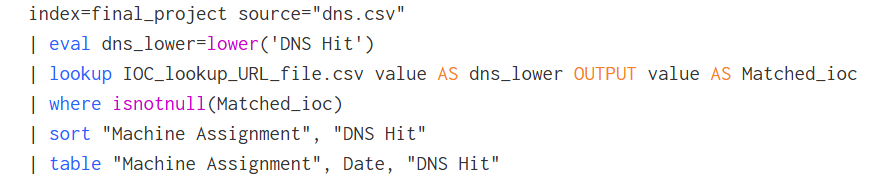
\includegraphics[width=0.8\textwidth]{SS_01}}
		\caption{DNS Log Query for IOC Matching}
		\label{fig: A1}
	\end{figure}
	
	\begin{figure}[h]
		\centering
		\fbox{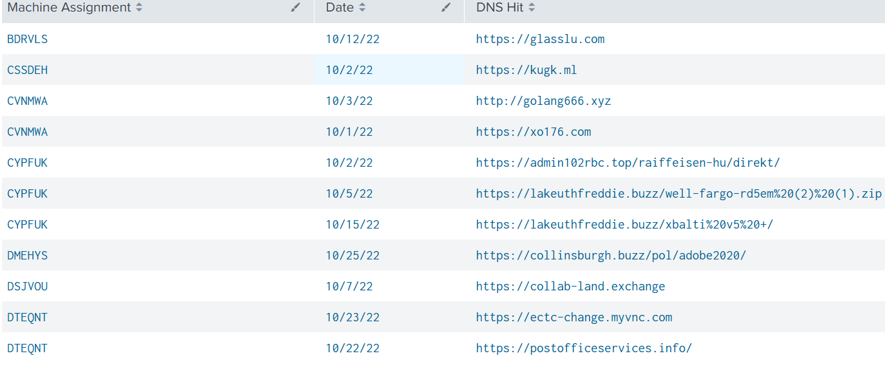
\includegraphics[width=0.8\textwidth]{SS_02}}
		\caption{Matched DNS Hits with Known Malicious Domains}
		\label{fig: A2}
	\end{figure}
	
	\begin{figure}[h]
		\centering
		\fbox{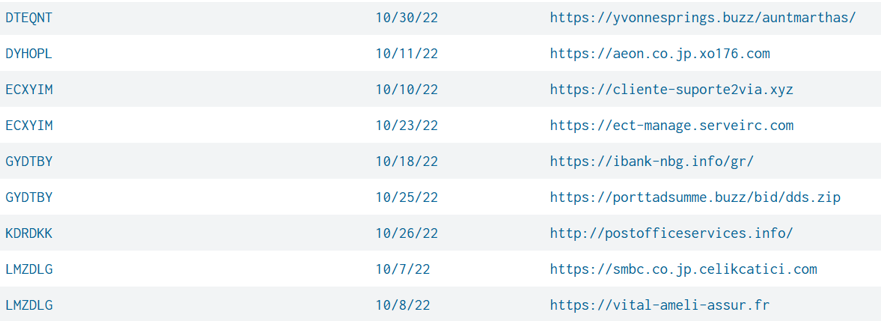
\includegraphics[width=0.8\textwidth]{SS_03}}
		\caption{Additional DNS Hits to Malicious Domains}
		\label{fig: A3}
	\end{figure}
	
	\begin{figure}[h]
		\centering
		\fbox{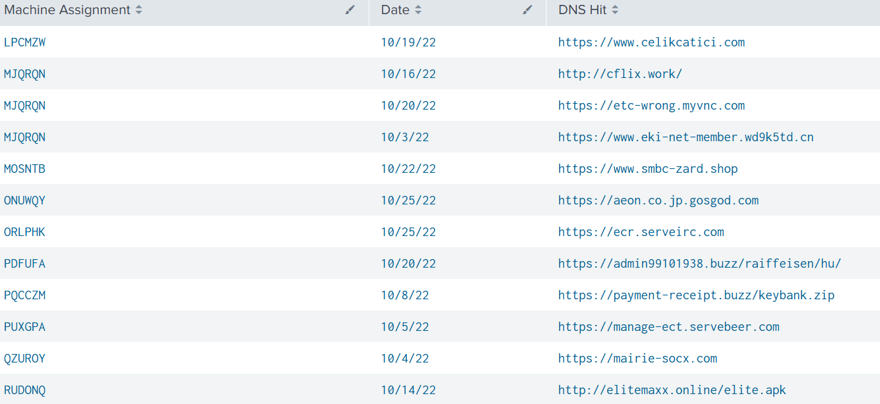
\includegraphics[width=0.8\textwidth]{SS_04}}
		\caption{Continued DNS Activity from Multiple Hosts to IOC-Flagged Domains}
		\label{fig: A4}
	\end{figure}
	
	\begin{figure}[h]
		\centering
		\fbox{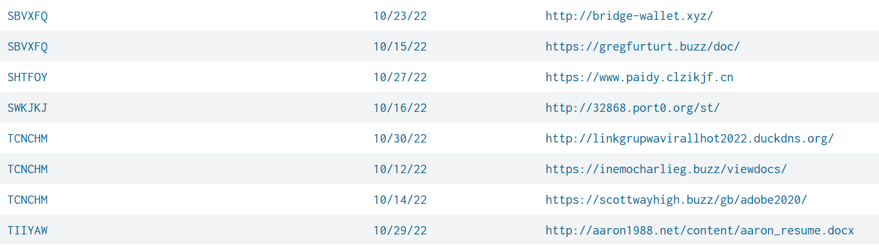
\includegraphics[width=0.8\textwidth]{SS_05}}
		\caption{DNS Hits to Malicious Domains Continued}
		\label{fig: A5}
	\end{figure}
	
	\begin{figure}[h]
		\centering
		\fbox{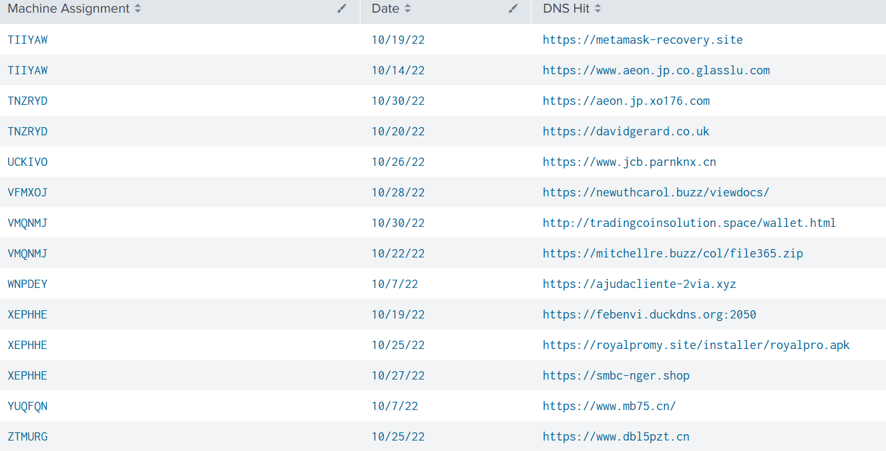
\includegraphics[width=0.8\textwidth]{SS_06}}
		\caption{Additional Malicious Domain Hits}
		\label{fig: A6}
	\end{figure}
	
	\begin{figure}[h]
		\centering
		\fbox{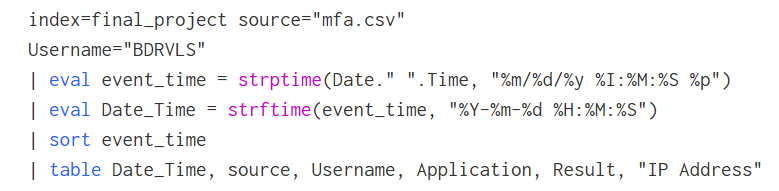
\includegraphics[width=0.8\textwidth]{SS_07}}
		\caption{MFA Log Query for USer BDRVLS}
		\label{fig: A7}
	\end{figure}
	
	\begin{figure}[h]
		\centering
		\fbox{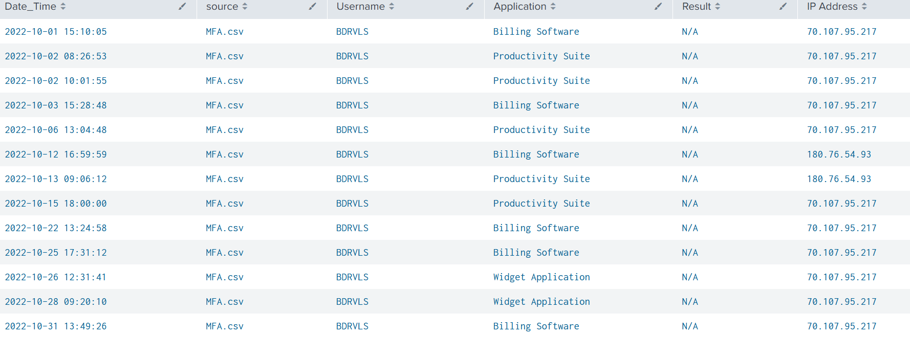
\includegraphics[width=0.8\textwidth]{SS_08}}
		\caption{MFA Log Events for User BDRVLS}
		\label{fig: A8}
	\end{figure}
	
	\begin{figure}[h]
		\centering
		\fbox{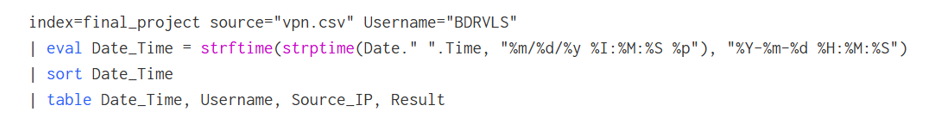
\includegraphics[width=0.8\textwidth]{SS_09}}
		\caption{VPN Log Query for User BDRVLS}
		\label{fig: A9}
	\end{figure}
	
	\begin{figure}[h]
		\centering
		\fbox{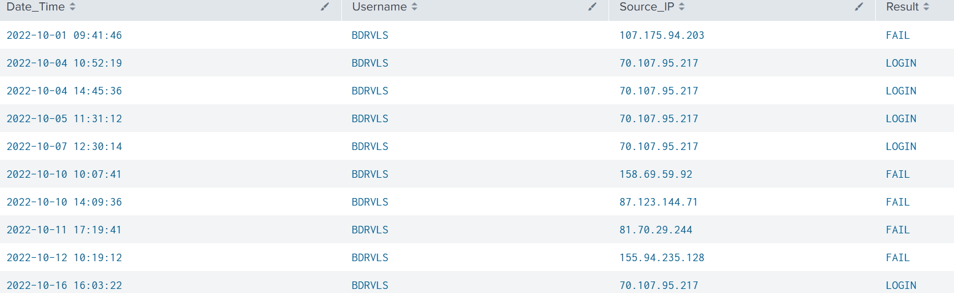
\includegraphics[width=0.8\textwidth]{SS_10}}
		\caption{Login Attempts for User BDRVLS with Multiple External IP}
		\label{fig: A10}
	\end{figure}
	
	\begin{figure}[h]
		\centering
		\fbox{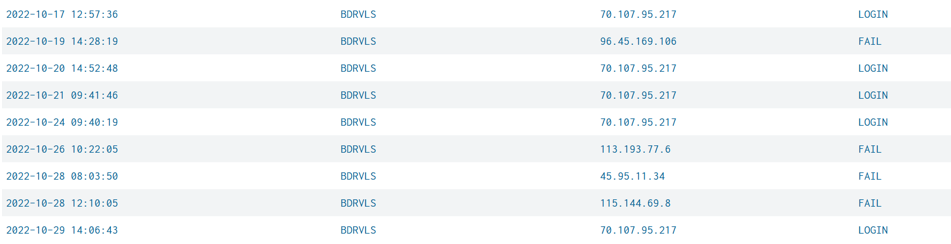
\includegraphics[width=0.8\textwidth]{SS_11}}
		\caption{VPN Login Activity for User BDRVLS}
		\label{fig: A11}
	\end{figure}
	
	\begin{figure}[h]
		\centering
		\fbox{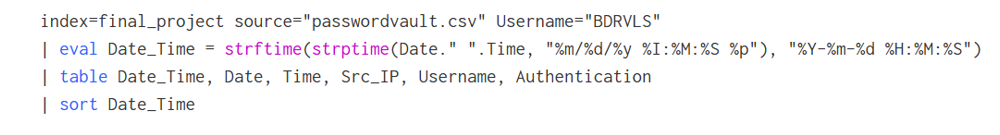
\includegraphics[width=0.8\textwidth]{SS_12}}
		\caption{Password Vault Log Query for User BDRVLS}
		\label{fig: A12}
	\end{figure}
	
	\begin{figure}[h]
		\centering
		\fbox{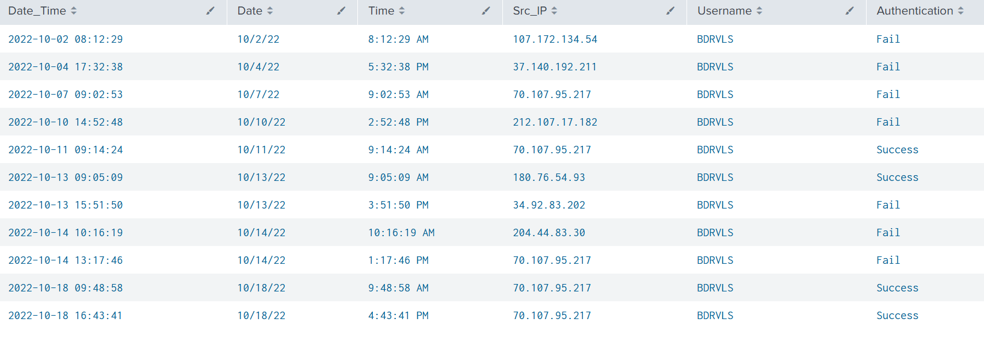
\includegraphics[width=0.8\textwidth]{SS_13}}
		\caption{Password Vault Access Attempts for User BDRVLS}
		\label{fig: A13}
	\end{figure}
	
	\begin{figure}[h]
		\centering
		\fbox{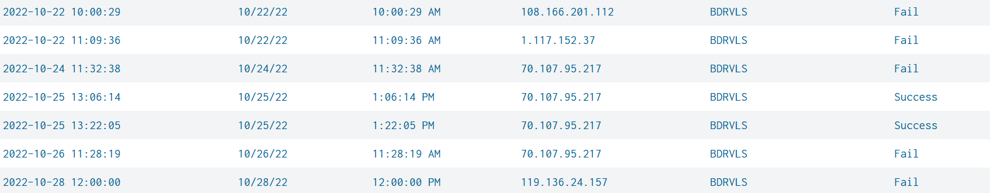
\includegraphics[width=0.8\textwidth]{SS_14}}
		\caption{Continued Password Vault Access Attempts}
		\label{fig: A14}
	\end{figure}
	
	\begin{figure}[h]
		\centering
		\fbox{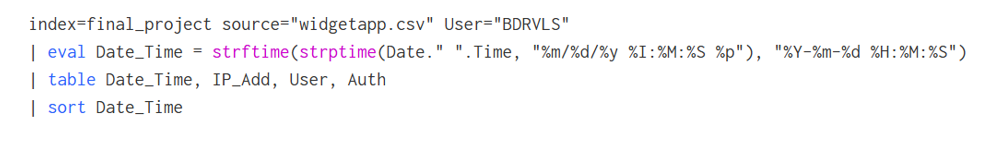
\includegraphics[width=0.8\textwidth]{SS_15}}
		\caption{WidgetApp Log Query for User BDRVLS}
		\label{fig: A15}
	\end{figure}
	
	\begin{figure}[h]
		\centering
		\fbox{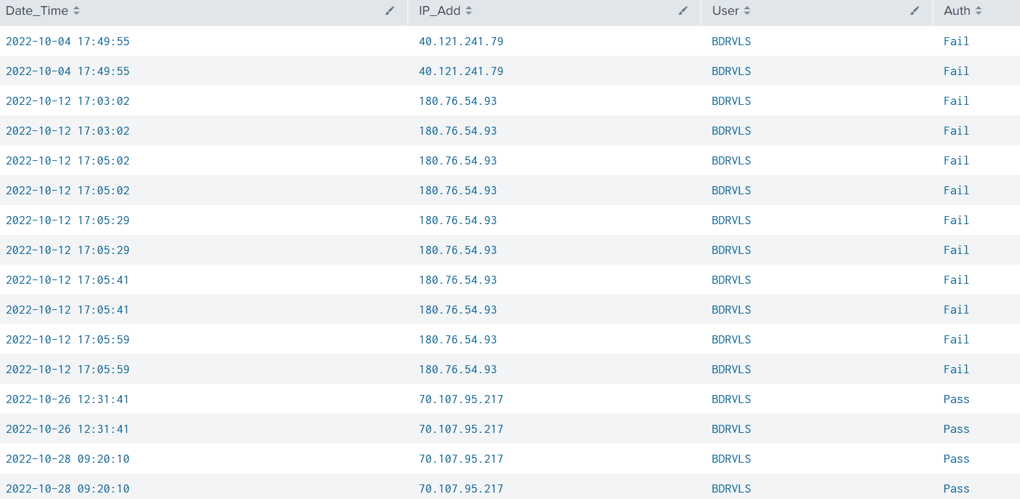
\includegraphics[width=0.8\textwidth]{SS_16}}
		\caption{WidgetApp Authentication Attempts for User BDRVLS}
		\label{fig: A16}
	\end{figure}
	
	\begin{figure}[h]
		\centering
		\fbox{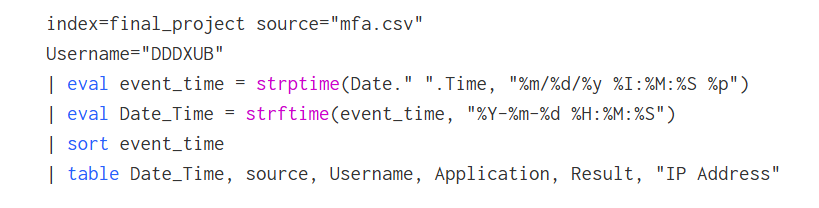
\includegraphics[width=0.8\textwidth]{SS_17}}
		\caption{MFA Log Query for User DDDXUB}
		\label{fig: A17}
	\end{figure}
	
	\begin{figure}[h]
		\centering
		\fbox{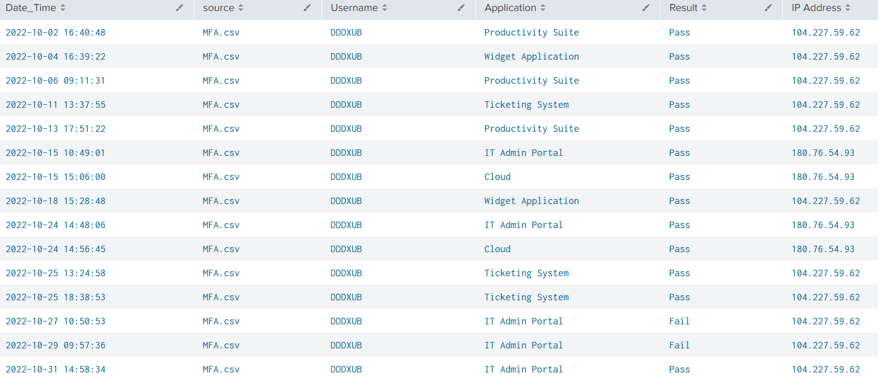
\includegraphics[width=0.8\textwidth]{SS_18}}
		\caption{MFA Log Activity for User DDDXUB}
		\label{fig: A18}
	\end{figure}
	
	\begin{figure}[h]
		\centering
		\fbox{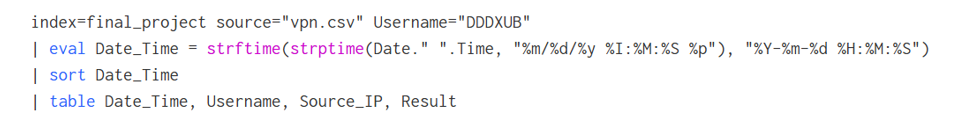
\includegraphics[width=0.8\textwidth]{SS_19}}
		\caption{VPN Log Query for User DDDXUB}
		\label{fig: A19}
	\end{figure}
	
	\begin{figure}[h]
		\centering
		\fbox{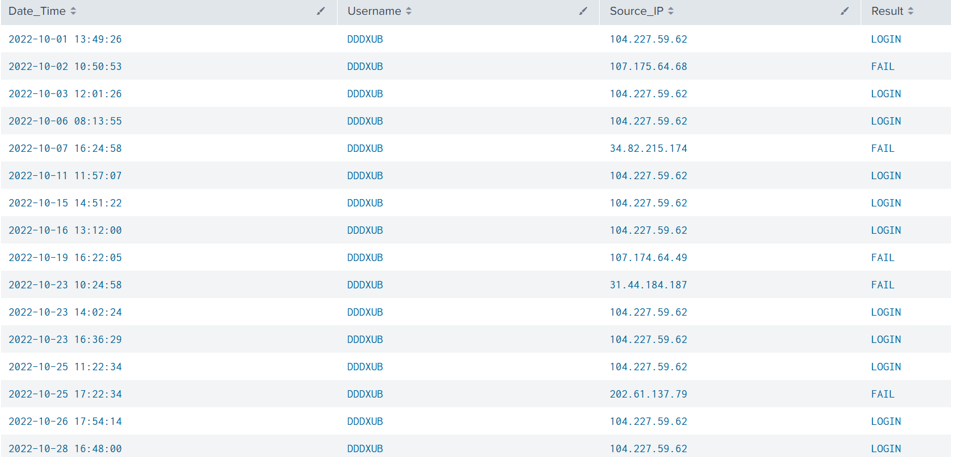
\includegraphics[width=0.8\textwidth]{SS_20}}
		\caption{VPN Login Activity for User DDDXUB with IOC IP Usage}
		\label{fig: A20}
	\end{figure}
	
	\begin{figure}[h]
		\centering
		\fbox{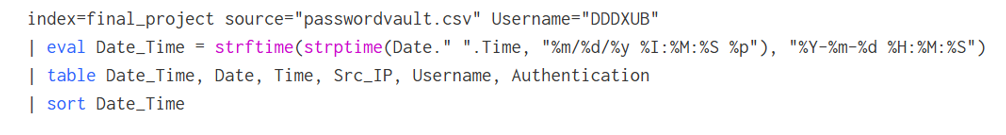
\includegraphics[width=0.8\textwidth]{SS_21}}
		\caption{Password Vault Log Query for User DDDXUB}
		\label{fig: A21}
	\end{figure}
	
	\begin{figure}[h]
		\centering
		\fbox{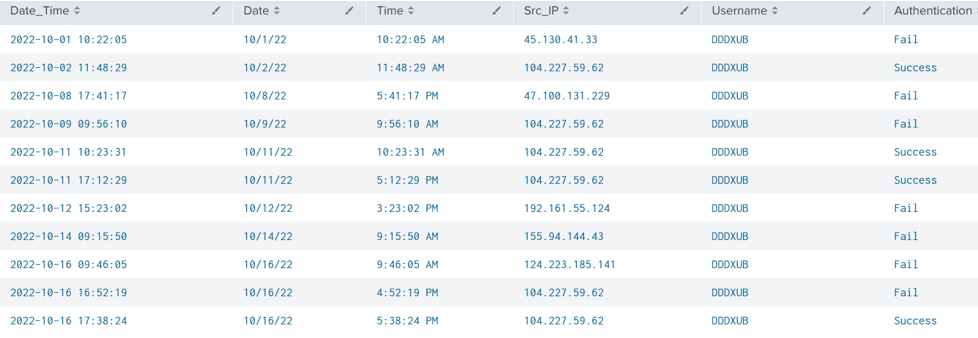
\includegraphics[width=0.8\textwidth]{SS_22}}
		\caption{Password Vault Access Attempts}
		\label{fig: A22}
	\end{figure}
	
	\begin{figure}[h]
		\centering
		\fbox{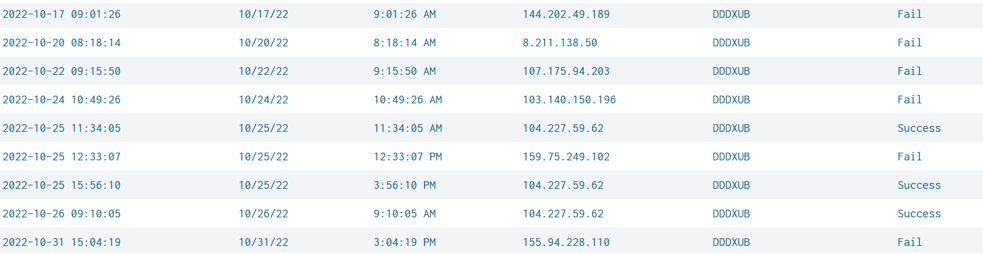
\includegraphics[width=0.8\textwidth]{SS_23}}
		\caption{Continued Password Vault Access Attempts for User DDDXUB}
		\label{fig: A23}
	\end{figure}
	
	\begin{figure}[h]
		\centering
		\fbox{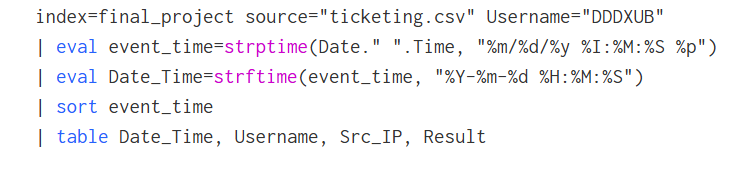
\includegraphics[width=0.8\textwidth]{SS_24}}
		\caption{Ticketing System Log Query for DDDXUB}
		\label{fig: A24}
	\end{figure}
	
	\begin{figure}[h]
		\centering
		\fbox{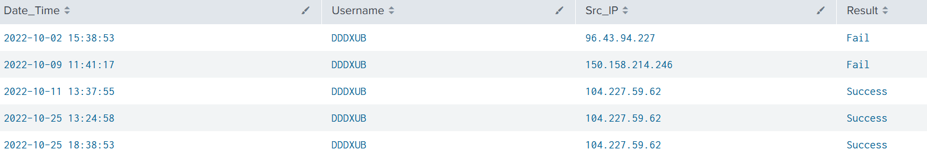
\includegraphics[width=0.8\textwidth]{SS_25}}
		\caption{Ticketing System Access Attempts}
		\label{fig: A25}
	\end{figure}
	
	\begin{figure}[h]
		\centering
		\fbox{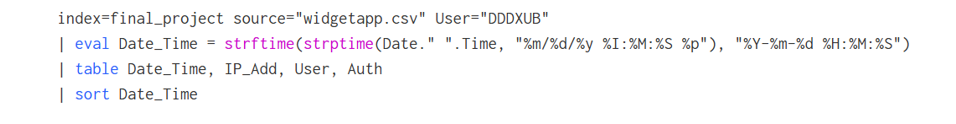
\includegraphics[width=0.8\textwidth]{SS_26}}
		\caption{WidgetApp Log Query for User DDDXUB}
		\label{fig: A26}
	\end{figure}
	
	\begin{figure}[h]
		\centering
		\fbox{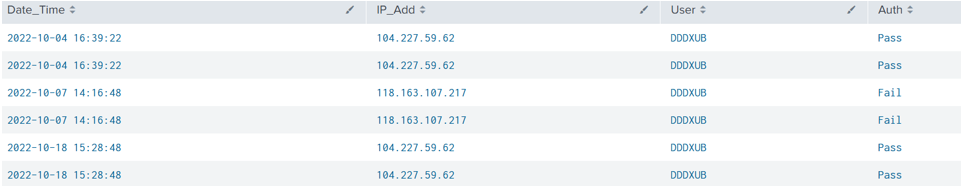
\includegraphics[width=0.8\textwidth]{SS_27}}
		\caption{WidgetApp Access Events for User DDDXUB}
		\label{fig: A27}
	\end{figure}
	
	\begin{figure}[h]
		\centering
		\fbox{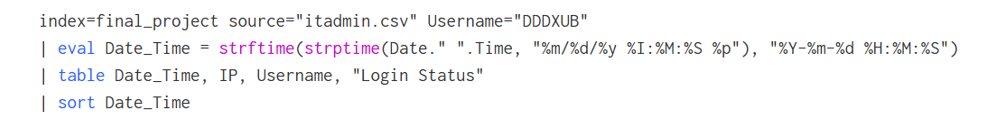
\includegraphics[width=0.8\textwidth]{SS_28}}
		\caption{IT Admin Portal Log Query for User DDDXUB}
		\label{fig: A28}
	\end{figure}
	
	\begin{figure}[h]
		\centering
		\fbox{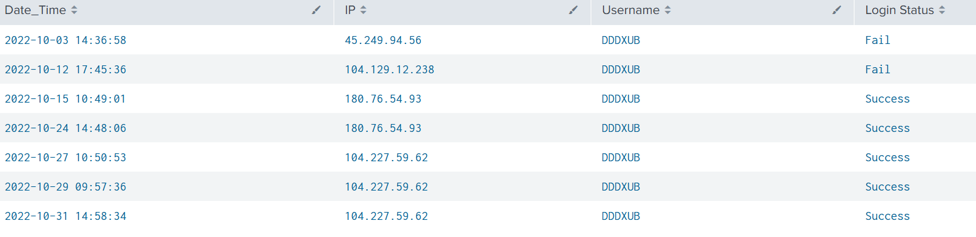
\includegraphics[width=0.8\textwidth]{SS_29}}
		\caption{IT Admin Portal Login Events for User DDDXUB}
		\label{fig: A29}
	\end{figure}

\FloatBarrier
\subsection{Dashboards and Insights}
	\renewcommand{\thefigure}{B\arabic{figure}}
	\setcounter{figure}{0}
	\begin{figure}[h]
		\centering
		\fbox{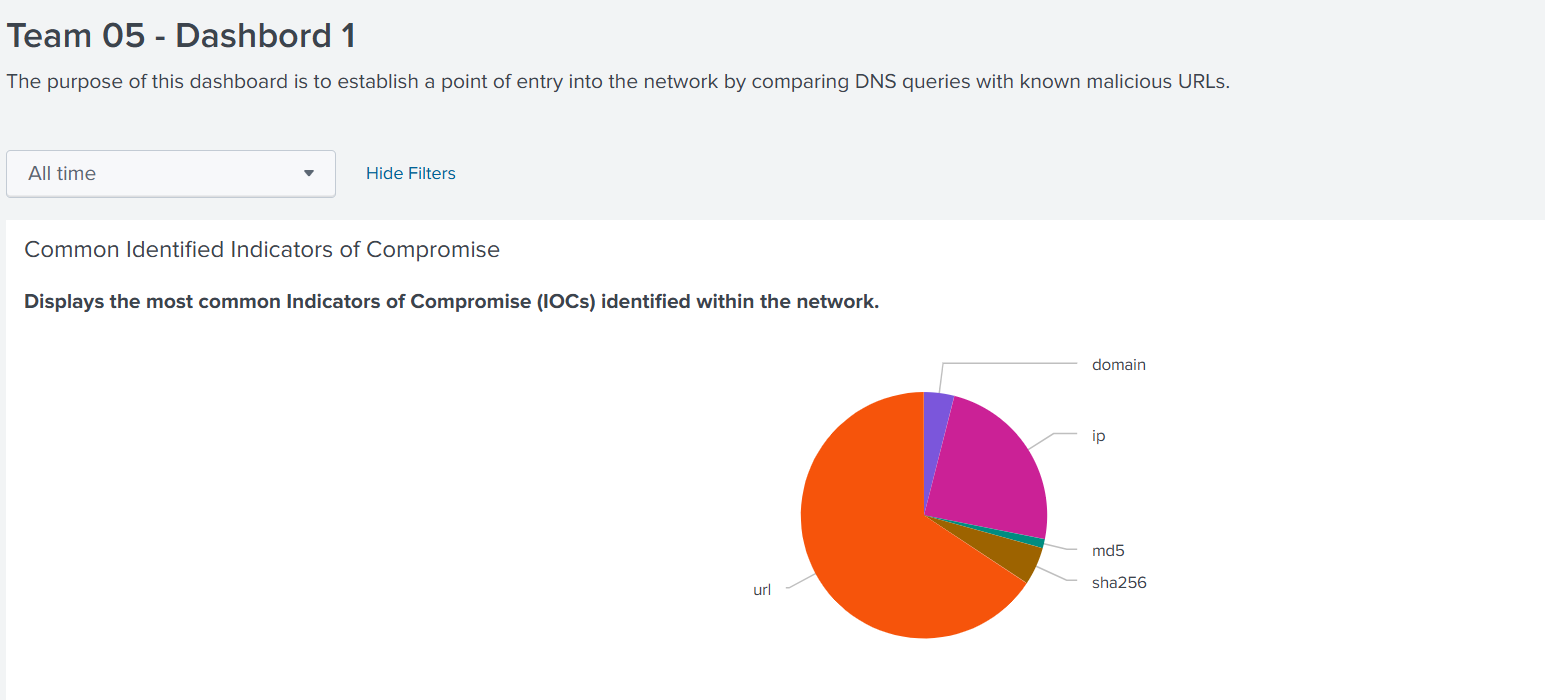
\includegraphics[width=0.8\textwidth]{SS_30}}
		\caption{Dashboard 01 – Entry Point Identification via DNS IOC Correlation}
		\label{fig: B1}
	\end{figure}
	
	\begin{figure}[h]
		\centering
		\fbox{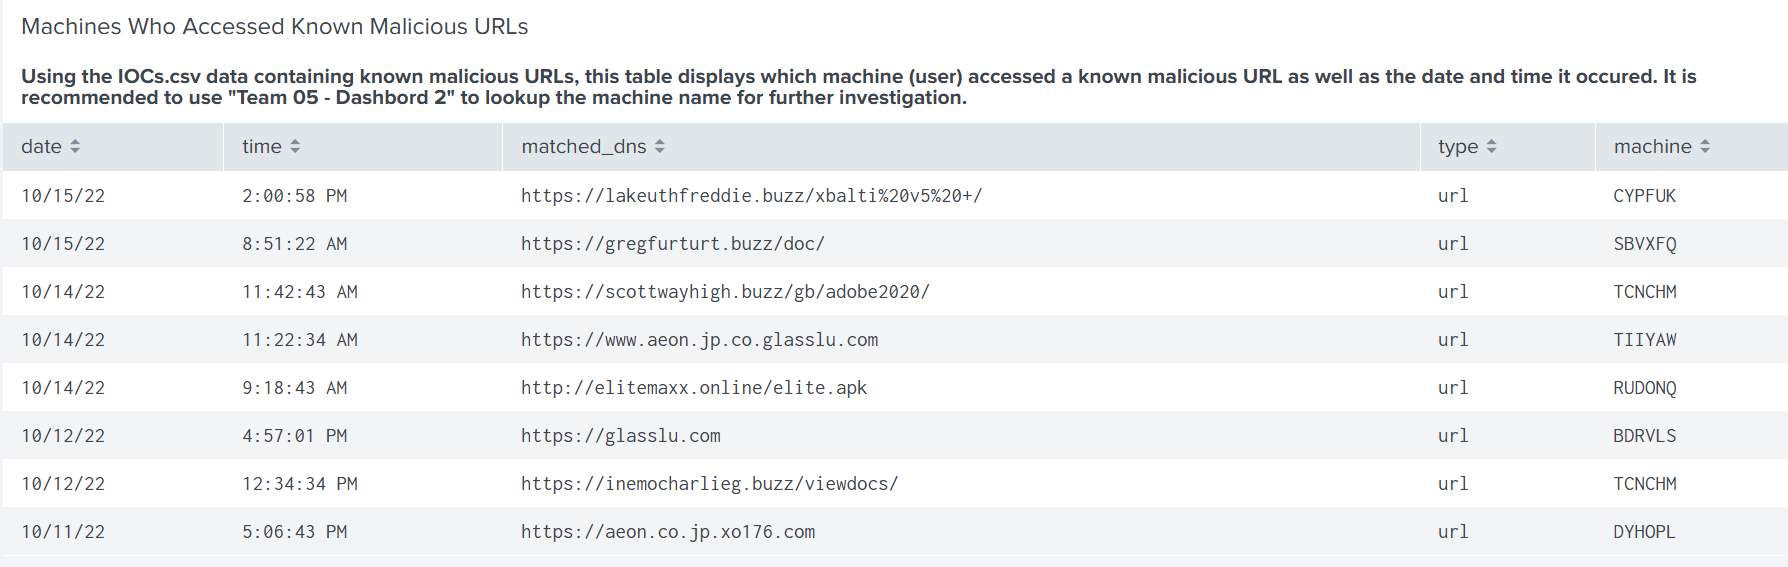
\includegraphics[width=0.8\textwidth]{SS_31}}
		\caption{Dashboard 01 – Table of Machines Accessing Known Malicious URLs}
		\label{fig: B2}
	\end{figure}
	
	\begin{figure}[H]
		\centering
		\fbox{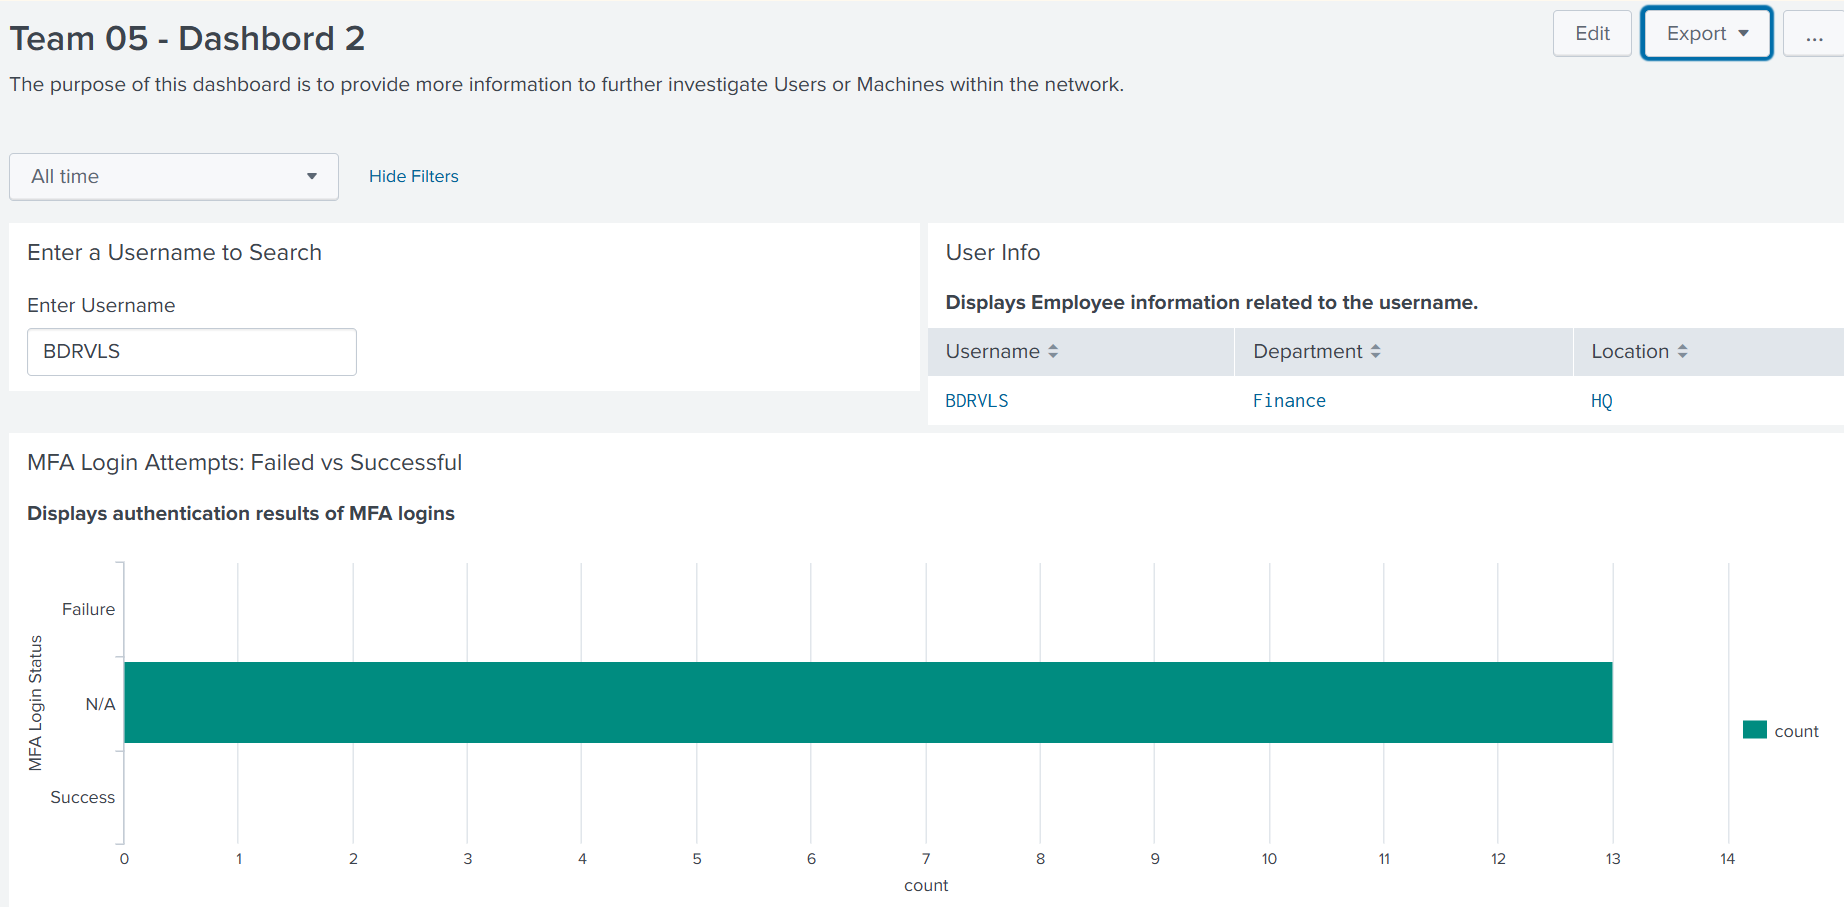
\includegraphics[width=0.8\textwidth]{SS_32}}
		\caption{Dashboard 02 - MFA Login Results for User BDRVLS}
		\label{fig: B3}
	\end{figure}
	
	\begin{figure}[h]
		\centering
		\fbox{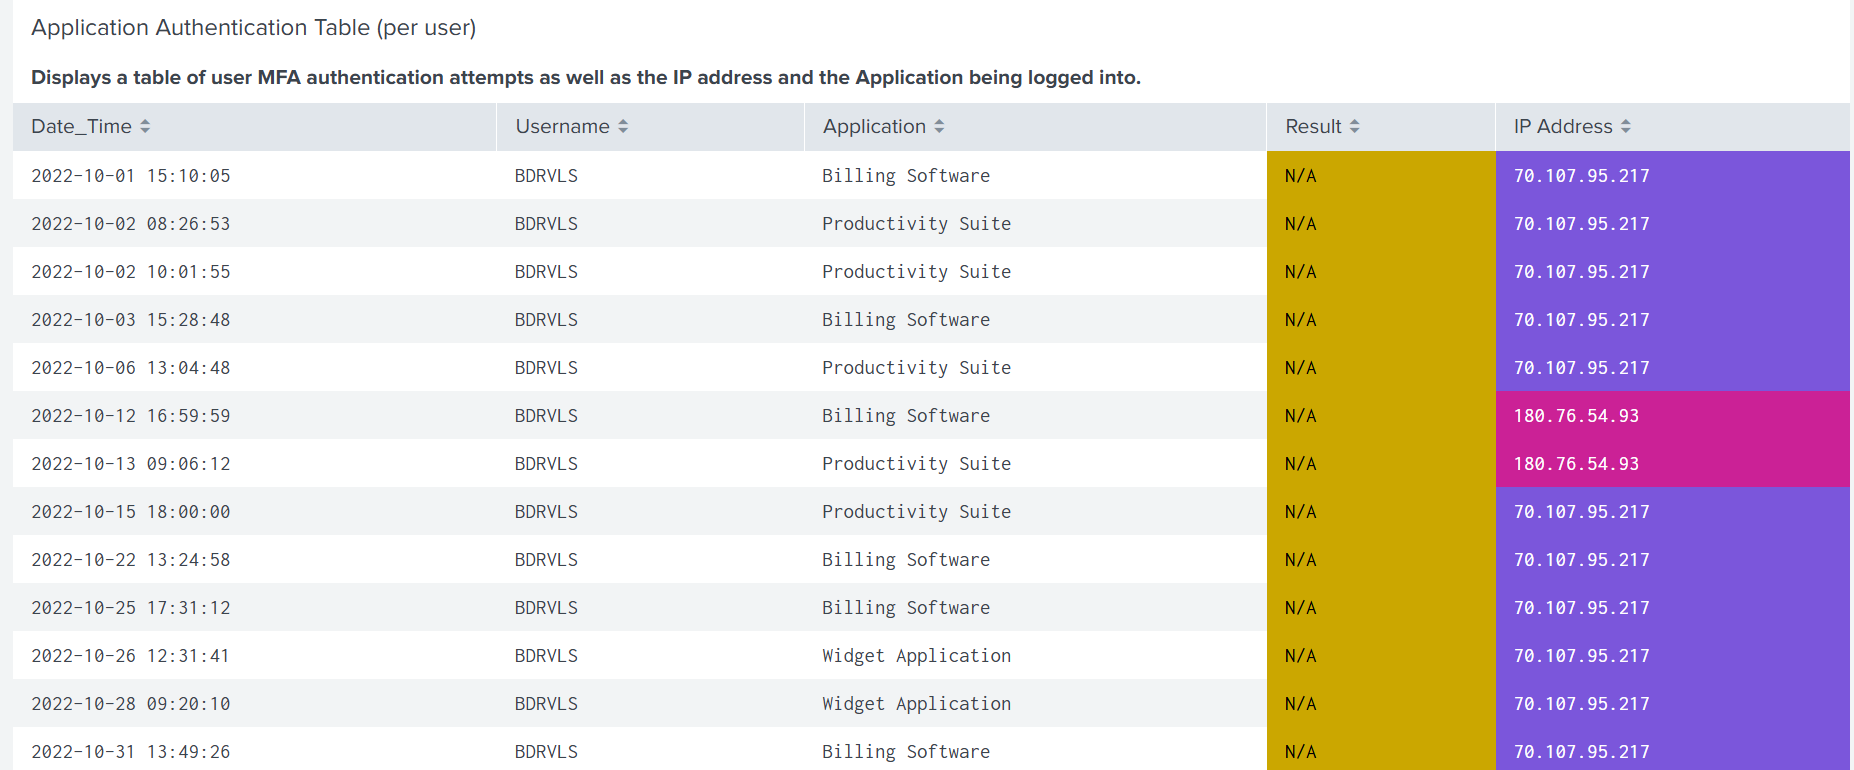
\includegraphics[width=0.8\textwidth]{SS_33}}
		\caption{Dashboard 02 - Authentication Activity for User BDRVLS}
		\label{fig: B4}
	\end{figure}
	
	\begin{figure}[h]
		\centering
		\fbox{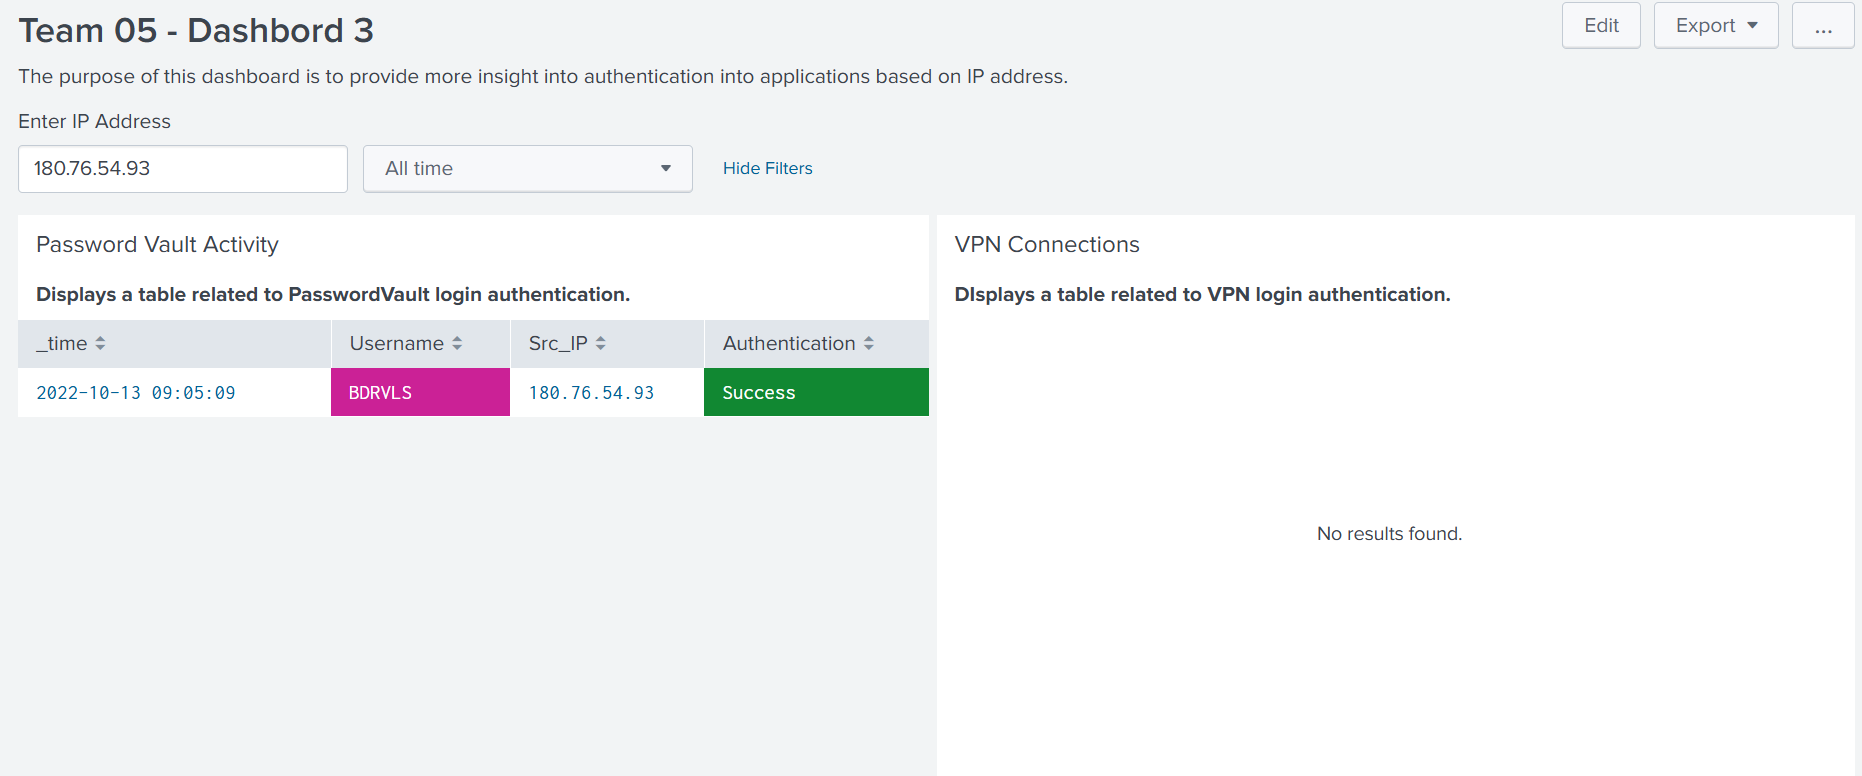
\includegraphics[width=0.8\textwidth]{SS_34}}
		\caption{Dashboard 03 - Password Vault Login from IOC-Tagged IP}
		\label{fig: B5}
	\end{figure}
	
	\begin{figure}[H]
		\centering
		\fbox{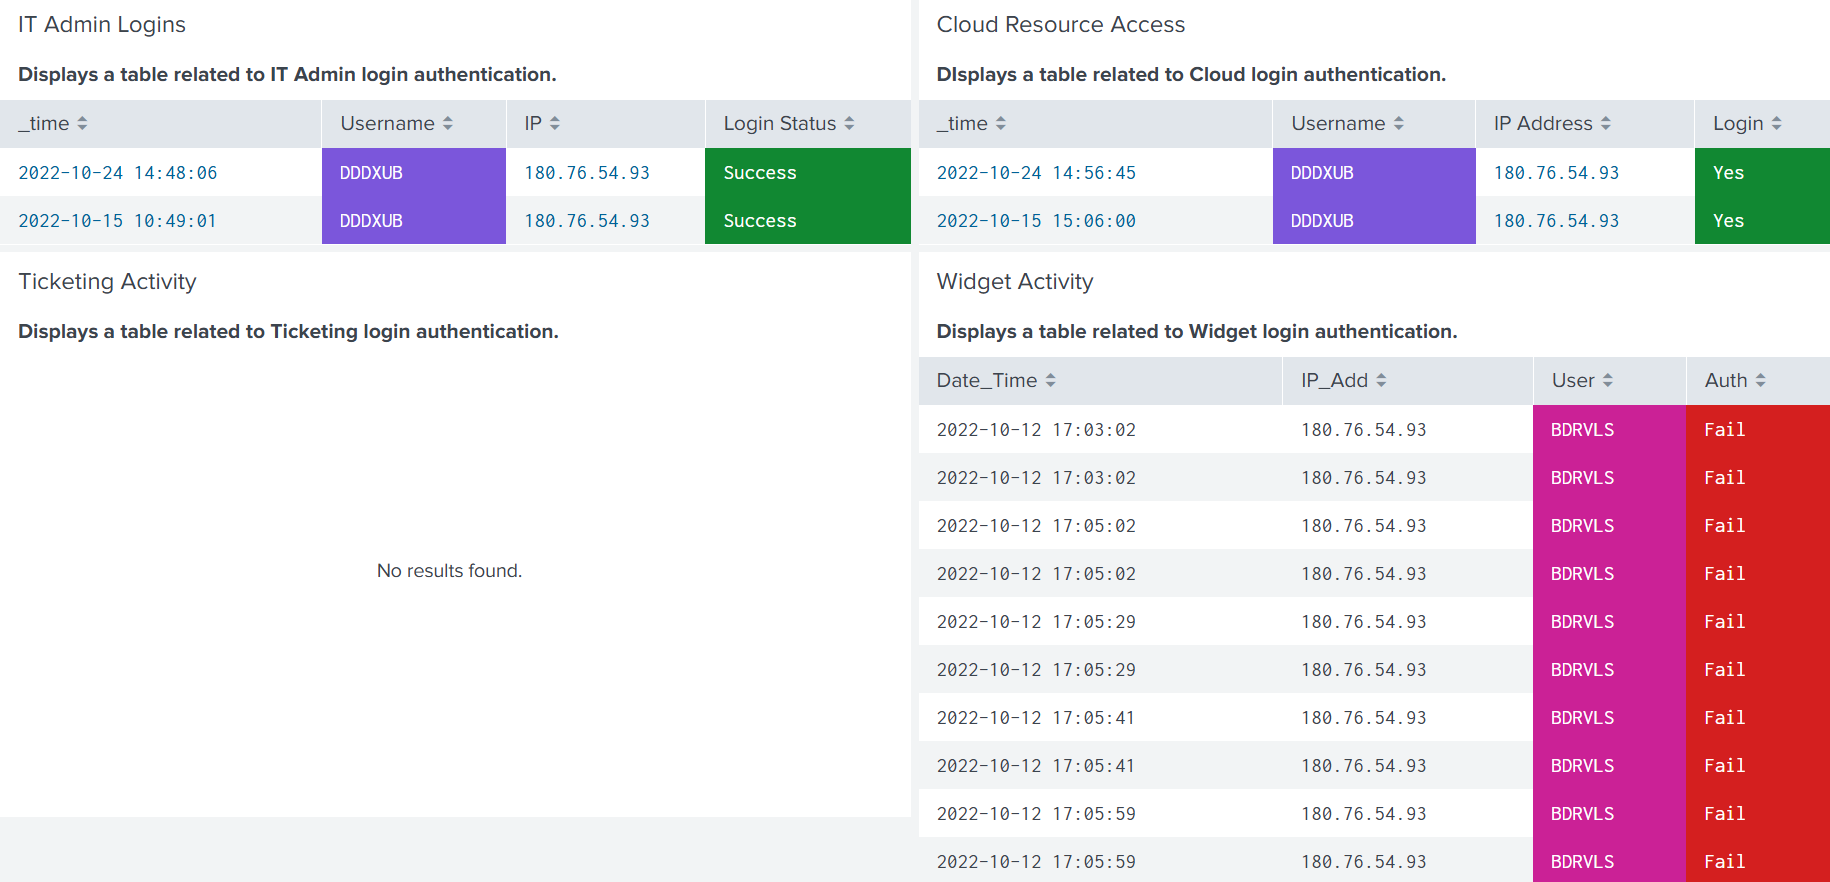
\includegraphics[width=0.8\textwidth]{SS_35}}
		\caption{Dashboard 03 - Correlation of IOC-Tagged IP Across Multiple Services}
		\label{fig: B6}
	\end{figure}
	

	
	
\end{document}